\documentclass{scrartcl}
% packages and settings for graphics
\usepackage[pdftex]{graphicx}
\graphicspath{{./}}
\DeclareGraphicsExtensions{.png}
\usepackage[final]{pdfpages}
\usepackage[margin=0.8in]{geometry}

\title{CSE705 Assignment 1 - Homework}
\begin{document}
\setcounter{secnumdepth}{0}
\setlength{\parskip}{10pt plus 1pt minus 1pt}

\section{Question 1}

\subsection{1}
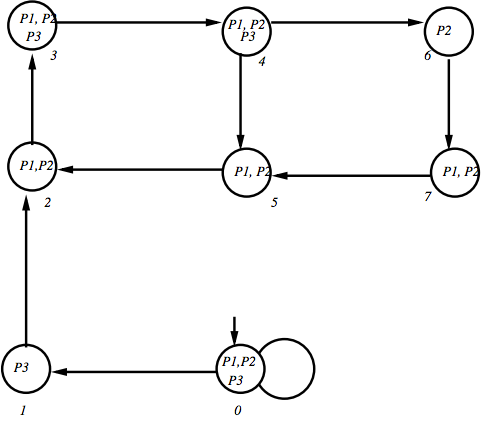
\includegraphics[width=3.6in]{q1model}
\newline
To verify the property $AF(\neg P1 \wedge \neg P2)$ we first need to transform it into the form of $EGf1$:

$\neg EG(\neg ( \neg P1 \wedge \neg P2)) \equiv \neg EG((P1 \vee P2))$.

We then apply the checkEG() algorithm: We identify states that satisfy $(P1 \vee P2)$: $S'$ = $\{0, 2, 3, 4, 5, 6, 7\}$
We form SCCs from these states = \{\{0\}, \{2, 3, 4, 5, 6, 7\}\}.
We pick an SCC and label all its states with $EG((P1 \vee P2))$.
We then perform backwards reachability and find that we can't find any other states in $S'$ that haven't been labeled and are reachable.
We label all other states with $\neg EG((P1 \vee P2))$ and we finish.

The final state of the model after performing checkEG() is:

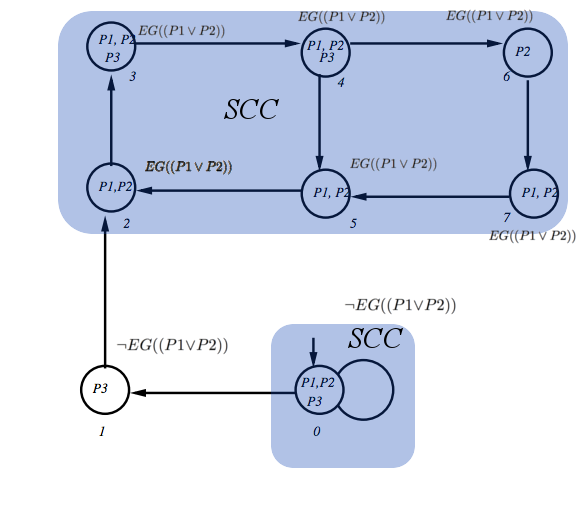
\includegraphics[width=3.6in]{q1modelchecked}

We can deterimine then that the model does not satisfy the property $AF(\neg P1 \wedge \neg P2)$

\subsection{2}
Mutual exclusion is a safety property: 
$AG(in\_critical\_section(0)  \oplus ...\oplus in\_critical\_section(n) \oplus critical\_section\_empty)$

Eventual entry to a critical section is a liveness property: $AG(AF(in\_critical\_section(0)) \wedge ... \wedge AF(in\_critical\_section(n)))$

Deadlock prevention : $AG(\forall (x, y) \in n \times n. \neg (waiting\_for(x, y) \wedge waiting\_for(y, x))$

\section{Question 2}
\section{Question 3}
\section{Question 4}
The difference between simulation and bisimulation is a question of where the observer is or what level of abstraction you are working with.

For example given two cars, one with an internal combustion engine and the other a hybrid vehicle. If we model them both as processes with states like driving and stopped and turning, and actions like drive, brake, turn, etc, both cars can simulate each other, and are bi-similar. The internal operations of how they achive these actions are different but from a driver's point of view they behave the same.

If we now go to a mechanics point of view, the hybrid vehicle has both a motor powered by internal combustion and electric motors. The other car has only a combustion engine. The hybrid car can perform all the actions that the car with the combustion engine can but not vice versa. We can say that the hybrid car simulates the other car.

\end{document}